\vspace{-2em}
\section{Introduction}
\label{sec:intro}
\vspace{-1em}

\begin{figure*}[t]
    \centering
\vspace{-3mm}
    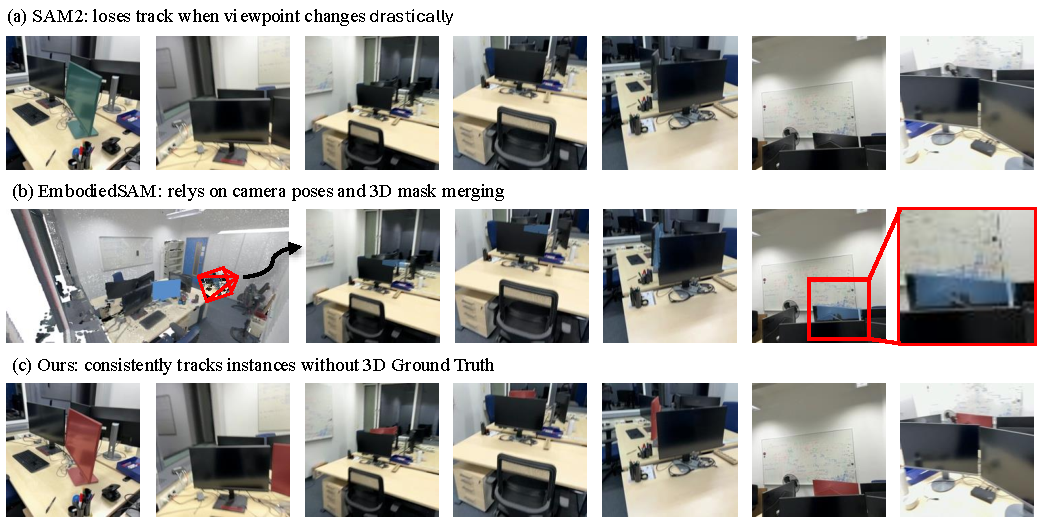
\includegraphics[width=\textwidth]{figs/comparison-teaser.pdf}
\vspace{-6mm}
    \caption{\textbf{Limitations of traditional VOS and 3D segmentation approaches, and an overview of our capability.}  
    (a) Traditional VOS methods such as SAM2~\cite{ravi2024sam2} lose track when the camera undergoes large viewpoint changes, causing masks to drift or disappear.  
    (b) 3D segmentation approaches rely on accurate camera poses and explicit 3D mask merging; they often propagate errors when the 3D reconstruction is incomplete or noisy.  
    (c) Our \textbf{3AM} consistently tracks object instances across drastic viewpoint changes without requiring camera poses or 3D ground-truth masks, demonstrating robust cross-view correspondence purely from geometry-aware 2D tracking.
    }
    \label{fig:intro-comparison}
\vspace{-3mm}
\end{figure*}

Video object segmentation (VOS) identifies and tracks target objects throughout a video sequence with consistent masks across frames. This is fundamental to autonomous driving, robotics, augmented reality, and video editing. A critical challenge is maintaining object identity under large viewpoint variations, temporary disappearances, or similar distractors. Traditional VOS methods rely on 2D appearance features and fail when the object appears dramatically different from varying viewpoints. For embodied AI in dynamic 3D environments, consistently recognizing objects across diverse viewpoints is essential for robust scene understanding.

Recent video object segmentation advances follow two parallel lines. First, 2D foundation models with memory-based architectures: SAM2~\cite{ravi2024sam2} introduced promptable segmentation with streaming memory and spatio-temporal attention. SAM2Long~\cite{ding2024sam2long} employs memory trees for long-range identity preservation, while DAM4SAM~\cite{videnovic2025distractor} incorporates distractor-aware updates. However, purely 2D approaches fail under large viewpoint changes as appearance features cannot establish reliable correspondence. Second, 3D instance segmentation methods: proposal-centric approaches like Mask3D~\cite{schult2022mask3d} and OneFormer3D~\cite{kolodiazhnyi2024oneformer3d} operate on point clouds, while projection-based methods like Open3DIS~\cite{nguyen2024open3dis}, SAM3D~\cite{yang2023sam3d}, and SAM2Object~\cite{zhao2025sam2object} lift 2D masks to 3D. These require camera poses, depth maps, preprocessing, and super-linear computational scaling.

Both paradigms have critical gaps (\cref{fig:intro-comparison}). 2D methods like SAM2 excel at efficiency but lack geometric awareness, failing under viewpoint variation (\cref{fig:intro-comparison}a). MOSEv2~\cite{ding2025mosev2} shows significant degradation under wide-baseline changes. Conversely, 3D methods achieve better consistency but require explicit 3D inputs (\cref{fig:intro-comparison}b) and struggle to generalize. 2D-to-3D lifting suffers from view-inconsistent predictions~\cite{jia2024sceneverse,peng2023openscene,takmaz2023openmask3d,xu2024embodiedsam,zhao2025sam2object}. End-to-end approaches like PanSt3R~\cite{zust2025panst3r} require offline processing. \emph{Can we achieve 3D-aware, viewpoint-robust segmentation while preserving promptability and efficiency, without explicit 3D supervision?} (\cref{fig:intro-comparison}c)

We introduce \textbf{3AM} (\cref{teaser}), a generalized 3D-aware tracker. Our key insight is that MUSt3R~\cite{cabon2025must3r} encodes implicit geometric correspondence through features learned from multi-view consistency. By fusing multi-level MUSt3R features with SAM2's appearance features via a lightweight Feature Merger, we enable geometry-consistent recognition based on spatial position, which at inference requires only RGB input and user prompts. We introduce a field-of-view aware sampling strategy ensuring frames observe spatially consistent object regions during training. On ScanNet++~\cite{yeshwanth2023scannet++} and Replica~\cite{replica19arxiv} with wide-baseline motion, 3AM achieves 90.6\% IoU and 71.7\% Positive IoU versus SAM2Long's 74.7\% and 41.3\% (+15.9 and +30.4 points).


In summary, our contributions are:
\begin{itemize}
\item \textbf{A key observation on the gap between 2D tracking and 3D consistency.}
2D tracking is fundamentally limited under large viewpoint variations. Existing 3D approaches require camera poses, depth, or 3D masks, often unavailable in practice. This motivates our geometry-aware framework, which achieves cross-view consistency without 3D supervision at inference.
\item \textbf{A 3D-aware feature integration framework} fusing geometric features from 3D reconstruction models with SAM2's appearance features, and \textbf{a field-of-view aware training strategy} ensuring geometric consistency for effective 3D correspondence learning.
\item \textbf{A generalized tracking framework} that adaptively reverts to the original SAM2 for non-rigid or highly dynamic objects, along with \textbf{extensive experimental evaluation} demonstrating consistent improvements over state-of-the-art VOS methods on challenging datasets such as ScanNet++ and Replica, especially under object reappearance and significant viewpoint changes, while retaining competitive performance on conventional VOS benchmarks.
\end{itemize}


